\documentclass[11pt, a4paper]{article}

\usepackage{graphicx}
\usepackage[a4paper,top=3cm,bottom=2cm,left=2cm,right=2cm,marginparwidth=1.75cm]{geometry}
\usepackage[english]{babel}
\usepackage[utf8x]{inputenc}
\usepackage{subfig}
\usepackage{float}
\usepackage{amsmath}
\usepackage{amssymb}
\usepackage{mhchem}
\usepackage{hyperref}
\usepackage{tikz}
\usepackage{cancel}

\graphicspath{ {./images} }
\renewcommand\epsilon{\varepsilon}
\newcommand*{\qed}{\hfill\ensuremath{\quad\square}}%
\newcommand*{\rad}{\ensuremath{\,\text{rad}}}
\newcommand*{\R}{\ensuremath{\mathbb{R}}}

\makeatletter
\renewcommand*\env@matrix[1][*\c@MaxMatrixCols c]{%
  \hskip -\arraycolsep
  \let\@ifnextchar\new@ifnextchar
  \array{#1}}
\makeatother

\newtheorem{theorem}{Theorem}

%------------------------------------------------
%Templates for images and figures
% \begin{figure}[h]
%   \centering
%   \subfloat[caption 1]{{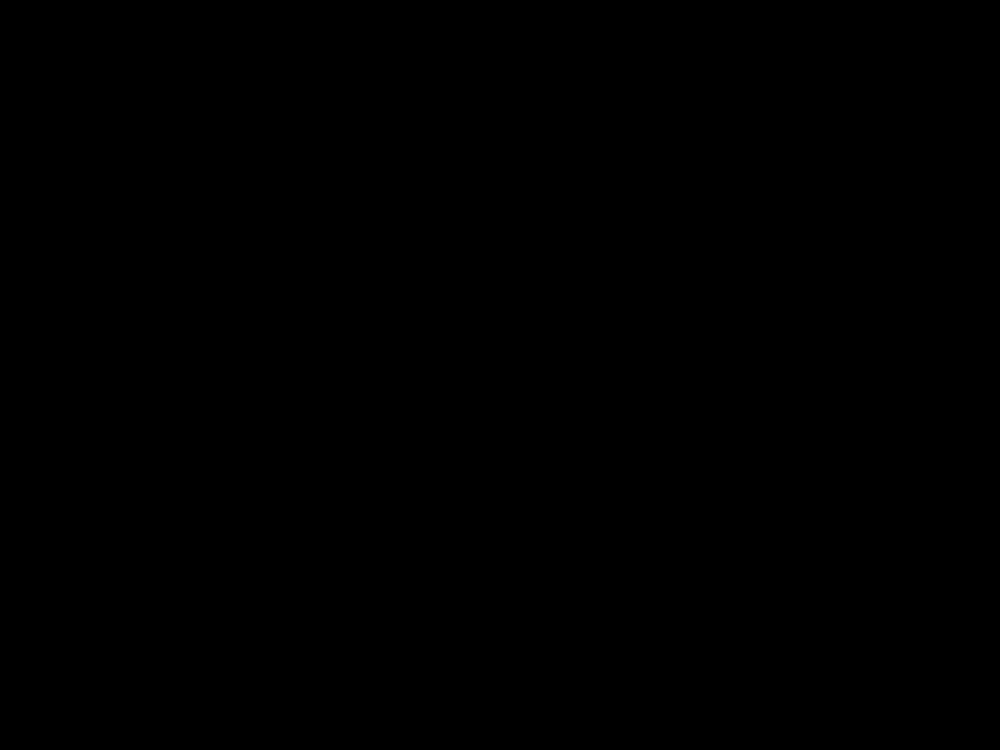
\includegraphics[width=30mm]{images/placeholder.png}}}%
%   \qquad
%   \subfloat[caption 2]{{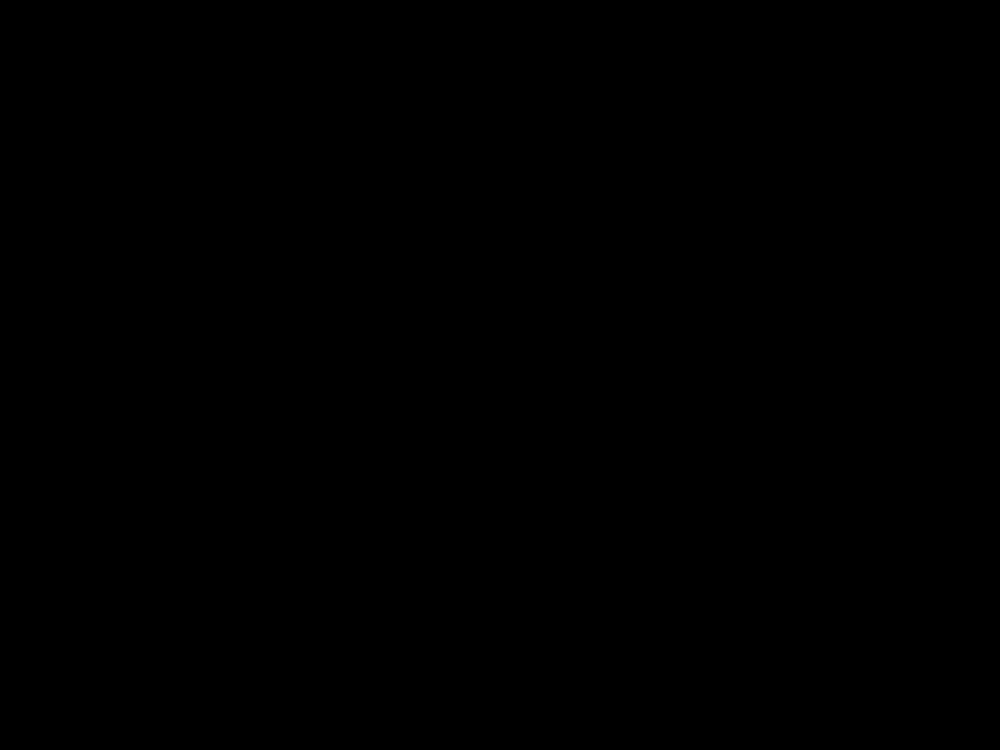
\includegraphics[width=30mm]{images/placeholder.png}}}%
%   \caption{Description}
% \end{figure}

% \begin{figure}[h]
%   \centerline{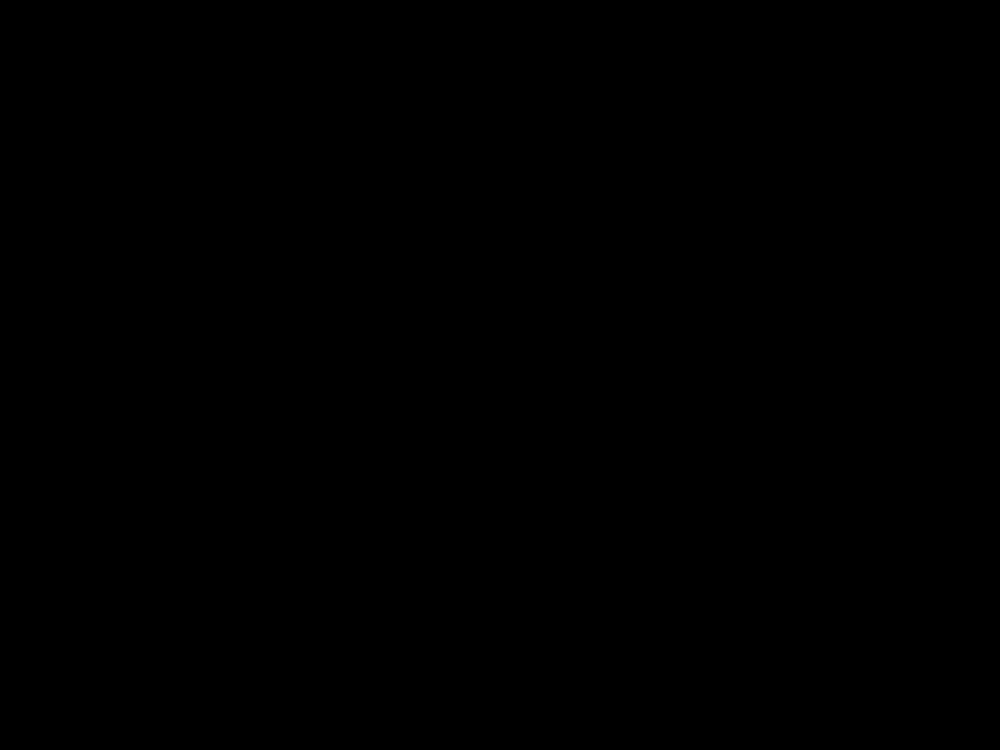
\includegraphics[width=50mm]{images/placeholder.png}}
%   \caption{Description}
% \end{figure}

%Template for a simple table 
%\begin{table}[h]
%   \caption{Description} %title of the table
%   \centering % centering table
%   \begin{tabular}{l rr} % creating three columns
%     \hline\hline %inserting double-line
%     & & \\ [0.5ex] % Insert half line vertical spacing
%     \hline % inserts single-line
%     & & \\ 
%     & & \\
%     & & \\
%     & & \\
%   \hline % inserts single-line
%   \end{tabular}
%   \label{tab:hresult}
% \end{table}
%-----------------------------------------------

\begin{document}
\setcounter{section}{7}
\setcounter{equation}{0}

\section{Thermofluid lecture 8: Non stationary control volumes and example systems}

\subsection{Non-stationary control volumes}
Recall the law of conservation of mass as it applies to an open system:
\begin{equation}
  \frac{dm_{CV}}{dt} = \sum_{in} \dot{m}_{in} - \sum_{out} \dot{m}_{out}
\end{equation}
When analyzing stationary control volumes we set the $\frac{dm_{CV}}{dt}$ term to $0$. For situations where the control volume is not volume setting this term to $0$ doesn't hold anymore. Instead we integrate both sides with respect to time:
\begin{equation*}
  \int_{0}^{t} \frac{dm_{CV}}{dt}\,dt = \int_{0}^{t} \sum_{in} \dot{m}_{in} \, dt - \int_{0}^{t} \sum_{out} \dot{m}_{out} \, dt
\end{equation*}
This equation then becomes:
\begin{equation}
  \label{eqn:consv_open_system}
  m_{CV}(t) - m_{CV}(0) = \sum_{in} m_{in} - \sum_{out} m_{out}
\end{equation}
Where equation \ref{eqn:consv_open_system} represents the conservation of mass law as it is applied to an open system with non-stationary control volume. This same idea also holds when considering the energy balance of the control volume. Recall the equation for energy balance of an open system with stationary control volume:
\begin{equation}
  \label{eqn:consv_energy}
  \frac{dE_{CV}}{dt} = \dot{Q}_{CV} - \dot{W}_{CV} + \sum_{in} \dot{m}_{in} \theta_{in} - \sum_{out} \dot{m}_{out} \theta_{out}
\end{equation}
Since the terms for $\Delta PE$ and $\Delta KE$ are often much smaller compared to internal energy we can approximate that $\frac{dE_{CV}}{dt} = \frac{dU_{CV}}{dt}$. When integrating equation \ref{eqn:consv_energy} with respect to time we end up with:
\begin{equation*}
  \int_{0}^{t} \frac{dE_{CV}}{dt} \,dt = \int_{0}^{t} \dot{Q}_{CV} \, dt - \int_{0}^{t} \dot{W}_{CV} \, dt + \int_{0}^{t} \sum_{in} \dot{m}_{in} \theta_{in} \, dt - \int_{0}^{t} \sum_{out} \dot{m}_{out} \theta_{out} \, dt
\end{equation*}
This integrates to the following equation:
\begin{equation}
  U_{CV}(t) - U_{CV}(0) = Q_{CV} - W_{CV} + \sum_{in} m_{in} \theta_{in} - \sum_{out} m_{out} \theta_{out}  
\end{equation}


\subsection{Example 1: Tank with pressure valve}
\begin{figure}[H]
  \centerline{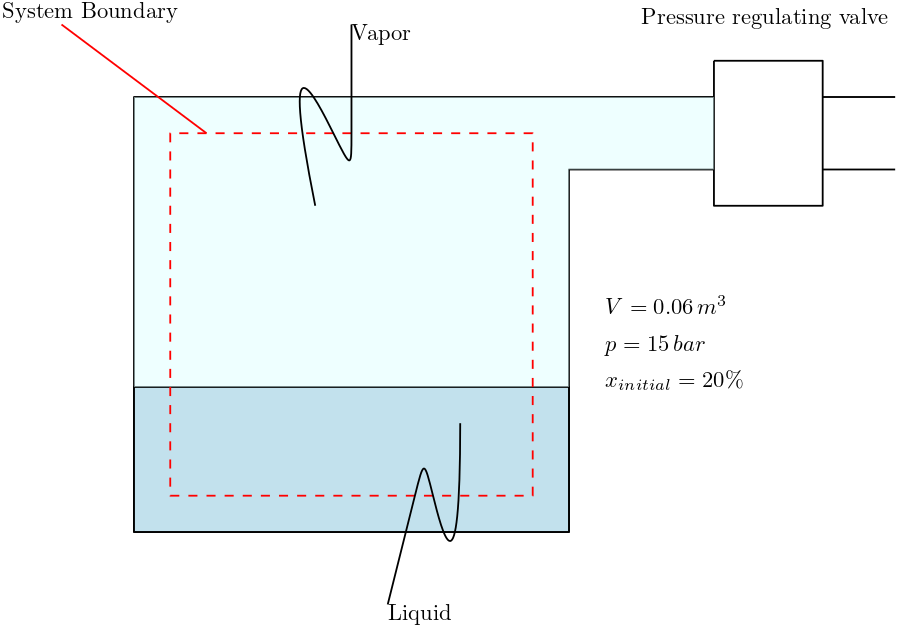
\includegraphics[width=80mm]{images/Tank.png}}
  \caption{The situation and initial conditions for the problem}
\end{figure}
The rigid tank contains an \ce{H2O} liquid-vapor mixture. The tank is kept at constant pressure with a pressure regulating valve. The valve allows satured vapor to escape the tank. Neglect the effects kinetic and potential energy. Find the total mass in $kg$ in the tank and the total amount of heat transfered in $kJ$ if heating continues untill the final quality of $x=50\%$.\\
We start by expressing the mass balance of the system:
\begin{gather*}
  \int_{0}^{t} \frac{dm_{CV}}{dt}\,dt = \int_{0}^{t} (\dot{m}_{in} - \dot{m}_{out})\,dt\\
  m_{CV}(t) - m_{CV,0} = - \int_{0}^{t} \dot{m}_{out} \, dt = \Delta m 
\end{gather*} 
Second we express the energy balance of the system:
\begin{equation*}
  \frac{dE_{CV}}{dt} = \dot{Q} - \dot{W} + \dot{m}_{in}\theta_{in} - \dot{m}_{out}\theta_{out}
\end{equation*}
We ignore the effects of kinetic and potential energy. This implies the following:
\begin{equation*}
  dE_{CV} \cong dU_{CV} \quad \text{and} \quad \theta \cong h
\end{equation*}
This gives us the following equation:
\begin{equation*}
  U(t) - U_0 = Q - \int_{0}^{t} \dot{m}_{out} h_{out}\, dt
\end{equation*}
$h_{out}$ stays constant over the valve. $\int_{0}^{t} \dot{m}_{out}$ has earlier been found to be equal to $-\Delta m$, thus:
\begin{equation*}
  U(t) - U_0 = Q + \Delta mh_{out}
\end{equation*}
$Q$ can then be expressed as:
\begin{gather*}
  Q = U(t) - U_0 - \Delta mh_{out}\\
  Q = m(t)u(t) - m_0u_0 - \Delta mh_{out}
\end{gather*}
We can now use either CoolProm or lookup tables in conjunction with interpolation to construct a table with all the relevant variables we need to find.
\begin{table}[h]
  \caption{The relevant values for the vapor quality $x$ and the corresponding specific volumes, specific internal energies and specific enthalpy.} %title of the table
  \centering % centering table
  \begin{tabular}{l rrr} % creating four columns
    \hline\hline %inserting double-line
    x & $v\,[m^3/kg]$ & $u\,[kJ/kg]$ & $h [kJ/kg]$\\ [0.5ex] % Insert half line vertical spacing
    \hline \hline% inserts double-line
    $0$   & $1.1539(10^{-3})$ & $843.16 $ & $-$\\ 
    $0.2$ & $0.02728$       & $1193.43$ & \\
    $0.5$ & $0.06648$       & $1718.83$ & \\
    $1$   & $0.1318$        & $2594.5$  & $2792.2$\\
  \hline % inserts single-line
  \end{tabular}
\end{table}
The intial mass of the system then becomes:
\begin{equation*}
  m_0 = \frac{V_0}{v_0} = \frac{0.06\,m^3}{0.02728\,m^3/kg} = 2.199\,kg
\end{equation*}
In this case time $t$ is when vapor quality equals $50\%$. The mass at time $t$ then becomes:
\begin{equation*}
  m_t = \frac{V}{v_t} = \frac{0.06\,m^3}{0.06648\,m^3/kg}=0.903\,kg
\end{equation*}
The value of $Q$ for the total amount of heat added then becomes:
\begin{align*}
  Q &= 0.903\,kg\cdot 1718.83\,kJ - 21.99\,kg\cdot 1193.43\,kJ - (0.903 - 2.199)\,kg \cdot 2792.2\,kJ\\
    &= 2547.2\,kJ
\end{align*}


\subsection{Example 2: Maximum efficiency of a wind turbine}
\begin{figure}[H]
  \centerline{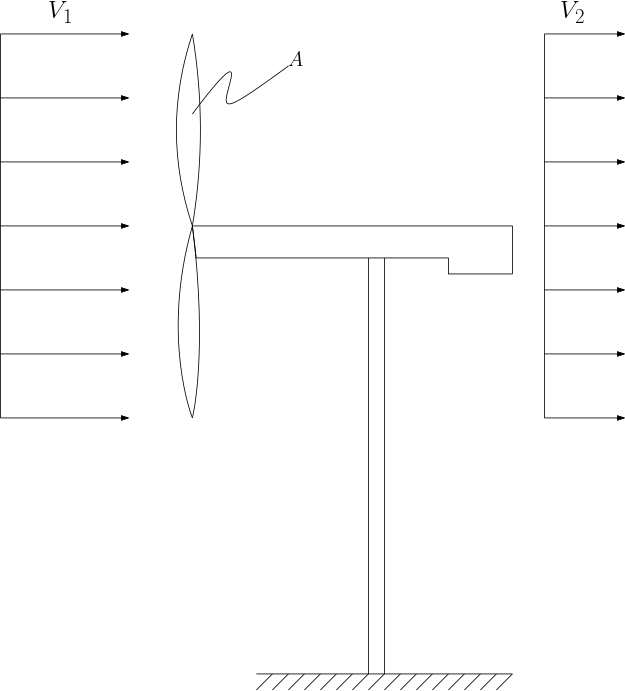
\includegraphics[width=80mm]{images/Turbine.png}}
  \caption{The turbine we are considering for the analysis}
  \label{fig:turbine}
\end{figure}
We are interested in finding the efficiency of the wind turbine in figure \ref{fig:turbine}. This efficiency can be expressed as the ration between work being done by the system and the kinetic energy of the wind going into the system.
\begin{equation*}
  \epsilon = \frac{\dot{W}}{\dot{KE}} = \frac{\dot{W}}{\frac{1}{2}\dot{m}V_1^2} = \frac{\dot{W}}{\frac{1}{2}\rho A V_1^3}
\end{equation*}
We know that some fraction of the kinetic energy going into the system is turned into work. Because of this we can know for sure that $V_2>V_1$. The system with stationary control volume can then be chosen as it's show in figure \ref{fig:TurbineSystem}.
\begin{figure}[h]
  \centerline{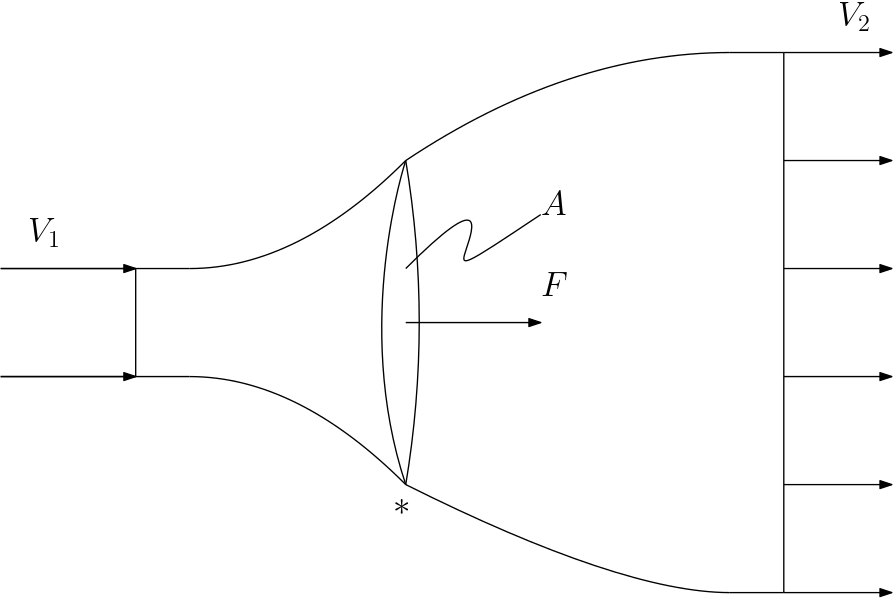
\includegraphics[width=80mm]{images/Turbine_System.png}}
  \caption{The system being considered for determening the efficiency $\epsilon$.}
  \label{fig:TurbineSystem}
\end{figure}
Applying the law of conservation of mass to this system gives the following relation:
\begin{equation*}
  \rho_1 V_1 A_1 = \rho_2 V_2 A_2 = \rho_* V_* A_*
\end{equation*}
Newton's second law of motion states that force is equal to the change of momentum over time. If we assume both mass and velocity to be time dependent and we apply the product rule we will find that:
\begin{equation*}
  \frac{d(mV)}{dt} = m\cancelto{0}{\frac{dV}{dt}} + V\frac{dm}{dt}
\end{equation*}
Note that the change in velocity with respect to time cancels to $0$ because the velocity at point $1$ going into the system is in fact constant. Thus we end up with the following:
\begin{equation*}
  \frac{d(mV)}{dt} = \dot{m}V
\end{equation*}
Using this and the law of conservation of mass we find that the force $F$ acting on the blade of the turbine is the following:
\begin{equation*}
  F = -\rho_1 V_1 A_1 V_1 + \rho_2 V_2 A_2 V_2
\end{equation*}
Let's now consider the energy balance of the system:
\begin{equation*}
  \frac{dE}{dt} = \dot{Q} - \dot{W} + \sum_{in} \dot{m}_{in} \theta_{in} - \sum_{out} \dot{m}_{out} \theta_{out}
\end{equation*}
We assume that the system is stationary and that transfer of heat across the system boundaries does not occur. This implies that the temperature stays constant. Since enthalpy and temperature are related by the following relation: $dh = c_p\,dT$ we know that $c_p$ is a constant. Thus if $dT$ is also constant $h_1 = h_2$. We also ignore the effect of gravity acting on the system. The energy equation then becomes:
\begin{equation*}
  \cancelto{0}{\frac{dE}{dt}} = \cancelto{0}{\dot{Q}} - \dot{W} + \dot{m}\left( \left(\cancel{h_1} + \frac{V_1^2}{2} \right) - \left( \cancel{h_2} + \frac{V_2^2}{2} \right)\right)
\end{equation*}
This leaves us with:
\begin{equation*}
  \dot{W} = \dot{m} \left( \frac{V_1^2}{2} - \frac{V_2^2}{2} \right)
\end{equation*}
We can now conclude that the power obtained from the stream of air can be expressed as:
\begin{equation*}
  -FV_* = \dot{W}
\end{equation*}
Subsituting in the expressions for $F$, $\dot{W}$ and the conservation of mass relation we found earlier gives:
\begin{equation*}
  -(-\dot{m}V_1+\dot{m}V_2)V_* = \dot{m} \left( \frac{V_1^2}{2} - \frac{V_2^2}{2} \right)  
\end{equation*}
Which simplifies to:
\begin{equation*}
  V_* = \frac{V_1 + V_2}{2}
\end{equation*}
Thus the velocity at the point $*$ is exactly the average of $V_1$ and $V_2$. Returning to the equation for $\epsilon$ and filling in the values we found gives:
\begin{equation*}
  \epsilon = \frac{\dot{m}\left( \frac{1}{2}V_1^2 - \frac{1}{2}V_2^2 \right)}{\frac{1}{2}\rho A V_1^3} = \frac{V_*(V_1^2 - V_2^2)}{v_1^3} = \frac{(V_1 + V_2)(V_1^2 - V_2^2)}{2V_1^3}
\end{equation*}
For simplicity let's define the ration $\frac{V_2}{V_1}$ as the variable $r$. This gives the following equation for $\epsilon$:
\begin{equation*}
  \epsilon = \frac{1}{2}(1 + r - r^2 - r^3)
\end{equation*}
The maximum efficiency occurs when $\frac{d\epsilon}{dr} = 0$, thus:
\begin{equation*}
  \frac{d\epsilon}{dr} = \frac{1}{2}(1 - 2r - 3r^2) = 0
\end{equation*}
Solving for $r_{1,2}$ with the quadratic equation:
\begin{equation*}
  r_{1,2} = \frac{-2 \pm \sqrt{4 + 4\cdot 3}}{6} \Rightarrow r_1 = -1 \wedge r_2 = \frac{1}{3}
\end{equation*}
Thus the lowest efficiency occur at $r_1$ and the maximum efficiency occurs at $r_2$. Filling in the value for $\epsilon(r)$ gives:
\begin{equation*}
  \epsilon = 0.593 = 59.3\%
\end{equation*}
Thus this gives us an upper limit of the efficiency which can be achieved by a wind turbine. This value works out to be $59\%$.
\end{document}